% !TEX root = SegwayDoku.tex
\newpage
\renewcommand{\autoren}{Valentyn Chepil}

\section{Die Hinderniserkennung}
\subsection{Ultraschallsensor}
% \ref{bild_3} zuweisung auf Bild in Text.

\begin{figure}[!h]  % [h] bedeutet, dass das Bild genau an dieser Stelle im Text erscheint
	% mit width=... wird die Größe des Bildes in Prozent der Seitenbreite eingestellt
	\centering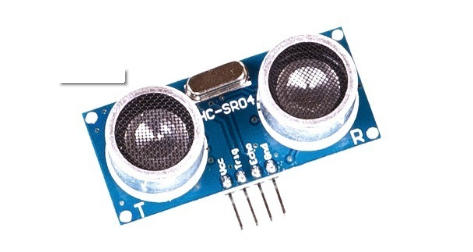
\includegraphics[width=0.5\textwidth]{images/Bild-1-1.png}
	% caption ist die Bildunterschrift, taucht auch im Abbildungsverzeichnis auf
	\caption{Ultraschallsensor \newline(Quelle: funduinoshop.com)}
	\label{bild_1.1} % über das label kann man aus dem Text auf das Bild verweisen
\end{figure}

Die Erkennung vom Hindernis erfolgt über ausgehenden Schallwellen, die sich in kegelförmig Form  ausbreiten. Bei Erreichung des Ziels werden die reflektierende Schallwellen aufgenommen und die Zeit des Reflektion wird ausgemessen. Dadurch erkennt man das Hindernis und den Abstand zu dem. Die Ausbreitung und die reflektierende Schallwellen hängt von verschiedenen Faktoren ab. Sie werden vom Luftdruck, der Umgebungstemperatur, der Luftfeuchtigkeit sowie vom Sende-/Empfangswinkel und der Oberfläche des im Schallkegel befindlichen Objekts beeinflusst.


\begin{figure}[!h]  % [h] bedeutet, dass das Bild genau an dieser Stelle im Text erscheint
	\centering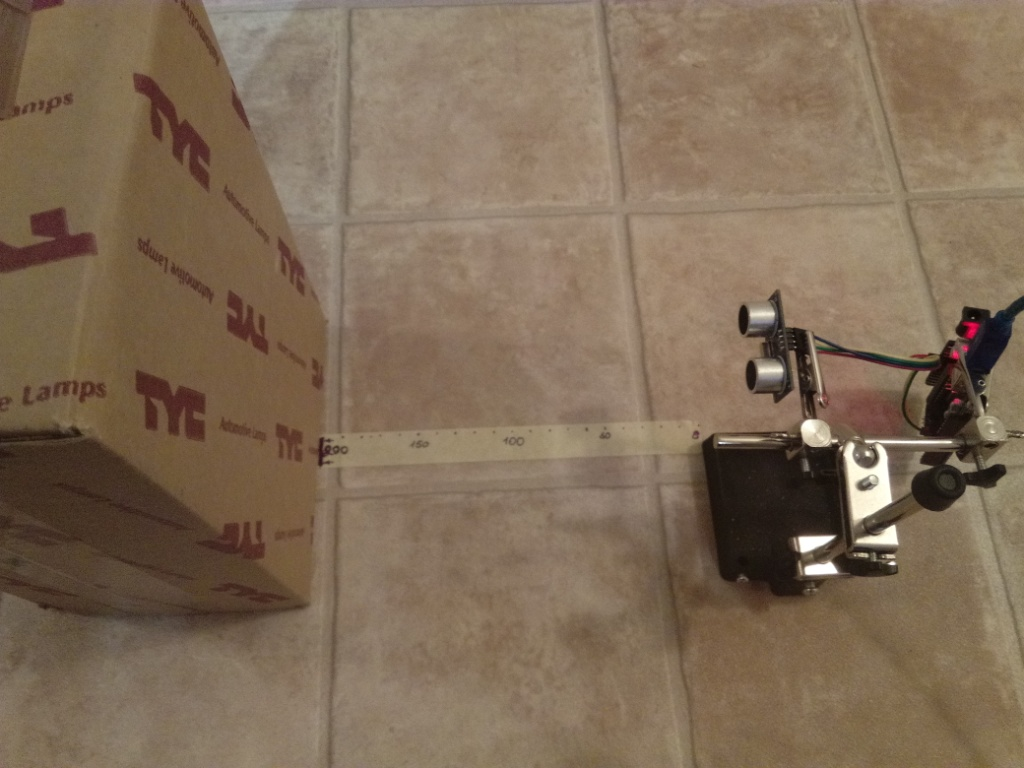
\includegraphics[width=0.6\textwidth]{images/Bild-1.jpg}
	\caption{Entfernungsmessung \newline (Quelle: eigene Darstellung, US-Sensor Messvorgang)}
	\label{bild_1} % über das label kann man aus dem Text auf das Bild verweisen
\end{figure}

\textbf{Vorteile:}  %fett 

Ein größter Vorteil des Ultraschallsensors ist günstiger Preis. Dies ermöglicht die Verwendung von vielen Sensoren bei der Modellbau, was zur präzisen Erfassung der Entfernung zu Hindernissen und die Objekte in der Umgebung führt. Die Abbildung \ref{bild_1} stellt ein Versuchsaufbau für Hinderniserkennen. 

\par\bigskip %leere zeile
\textbf{Nachteile:}  %fett 

Ein Hindernis oder Objekt kann nicht genau geortet werden, sondern man kann nur feststellen, dass es sich in der gemessenen Entfernung innerhalb des Schallkegels befindet. Kann man in der Abbildung \ref{bild_2} anschauen.

\begin{figure}[ht]  % [h] bedeutet, dass das Bild genau an dieser Stelle im Text erscheint
	\centering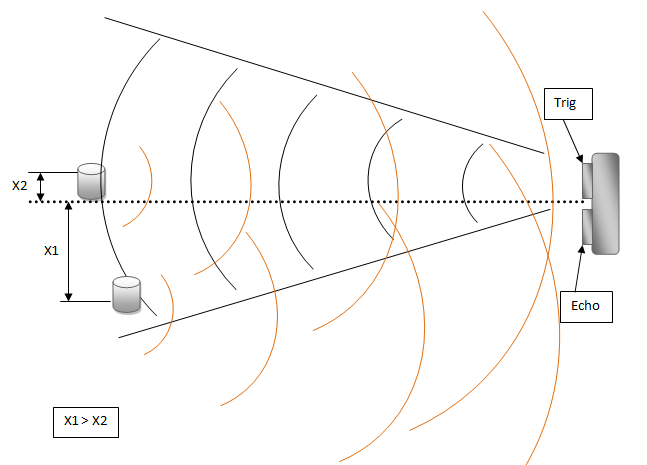
\includegraphics[width=0.6\textwidth]{images/Bild-2.png}
	\caption{Positionierung in Messbereich \newline (Quelle: eigene Darstellung)}
	\label{bild_2} % über das label kann man aus dem Text auf das Bild verweisen
\end{figure}

Bei mehrere Objekte vor Schallwelle wird der Abstand zum nächstliegenden Hindernis gemessen und die weit liegender Objekte werde einfach nicht erkannt. Das ist in der Abbildung \ref{bild_3} zu sehen.

\begin{figure}[ht]  % [h] bedeutet, dass das Bild genau an dieser Stelle im Text erscheint
	\centering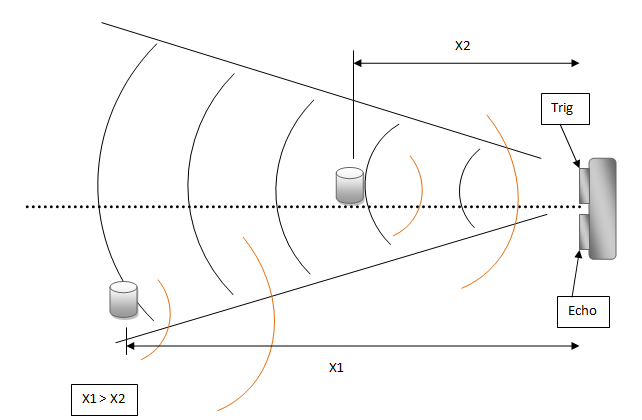
\includegraphics[width=0.6\textwidth]{images/Bild-3.png}
	\caption{Positionierung in Messbereich \newline (Quelle: eigene Darstellung)}
	\label{bild_3} % über das label kann man aus dem Text auf das Bild verweisen
\end{figure}

Als Nachteil kann man auch nennen, die geringe Reichweite (ca. 3m) des Ultraschalls und  der geringen Ausbreitungsgeschwindigkeit des Schalls, was bei  bewegenden Maschinen (im unserem Fall, Wackelroboter) zur Kollision mit Hindernis führen kann.

Große Probleme bekommt man auch aus den Reflektionseigenschaften der Schallwellen. Besonders bei weichen Materialien und spitzen-förmigen Oberflächen erkennt  der Sensor auch schleicht. Beispiel der Oberfläche kann man in der Abbildung \ref{bild_4} und \ref{bild_6} betrachten.

\begin{figure}[!h]  % [h] bedeutet, dass das Bild genau an dieser Stelle im Text erscheint
	\centering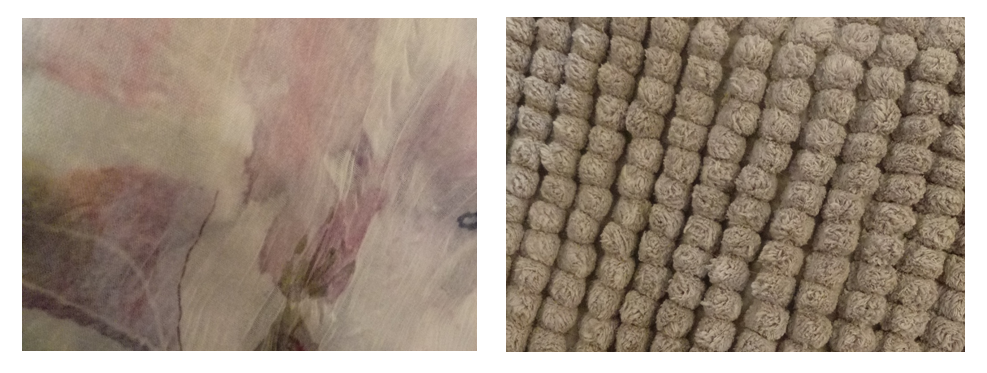
\includegraphics[width=0.7\textwidth]{images/Bild-4-5.png}
	\caption{Weiche und spitzen-förmige-weiche Oberflächen \newline(Quelle: eigene Darstellung,Frauen-Halsschal und Teppich)}
	\label{bild_4}
\end{figure}
\begin{figure}[!h]  % [h] bedeutet, dass das Bild genau an dieser Stelle im Text erscheint
	\centering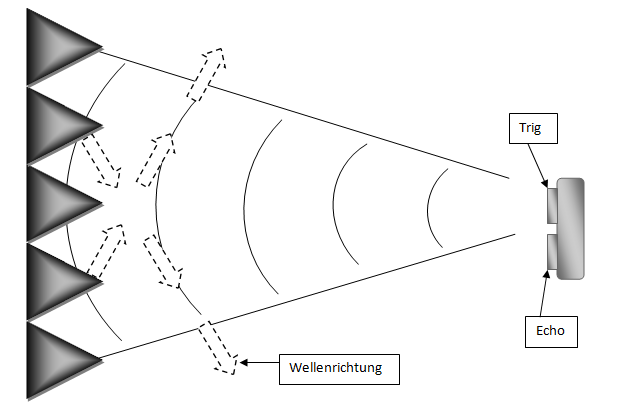
\includegraphics[width=0.6\textwidth]{images/Bild-6.png}
	\caption{Spitzen-förmige Oberflächen\newline(Quelle: eigene Darstellung, z.B: Kanten)}
	\label{bild_6}
\end{figure}

Wird den Öffnungswinkel bei Hindernis kleiner 75 Grad, so erreicht die Reflektion den aussendenden Sensor nicht (Bild \ref{bild_7}). 

\begin{figure}[!h]  % [h] bedeutet, dass das Bild genau an dieser Stelle im Text erscheint
	\centering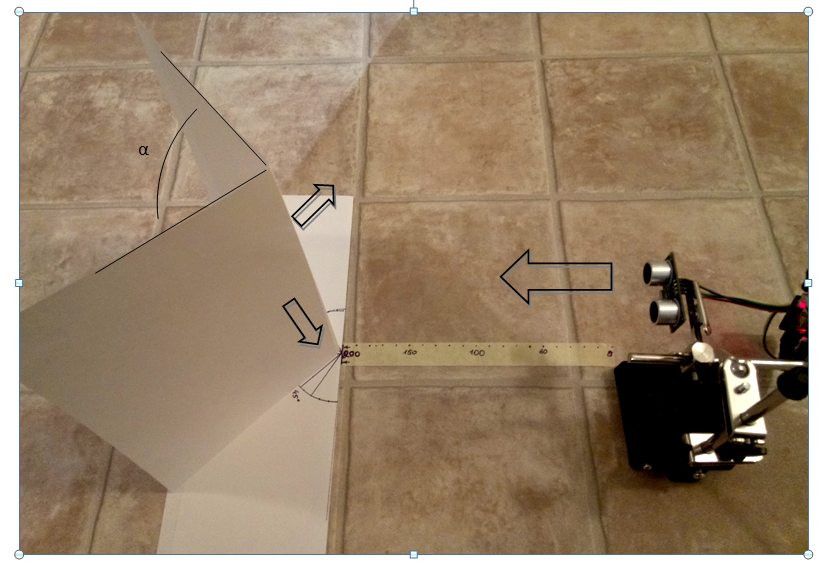
\includegraphics[width=0.6\textwidth]{images/Bild-7.png}
	\caption{Öffnungswinkel (Quelle: eigene Darstellung)}
	\label{bild_7} % über das label kann man aus dem Text auf das Bild verweisen
\end{figure}

Aus der Fähigkeiten des Sensors wurde folgenden Modul konstruiert und angepasst. Auf der Abbildung \ref{H-Mod} ist den Öffnungswinkel von drei US-Sensoren zu sehen.

\begin{figure}[!h]  % [h] bedeutet, dass das Bild genau an dieser Stelle im Text erscheint
	\centering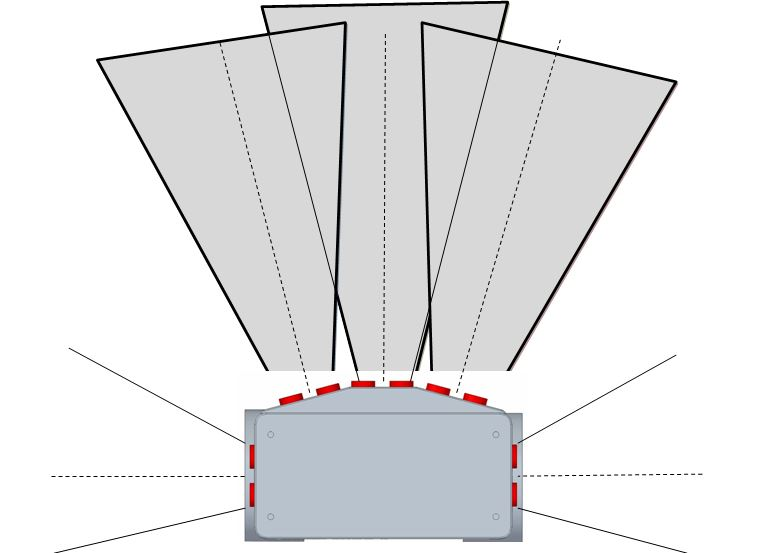
\includegraphics[width=0.95\textwidth]{images/H-Mod.jpg}
	\caption{Modul zur Hinderniserkennung mit Ultraschallsensoren (US1, US2, US22, US3, US33); mit US1 - Mitte, US2, US3 - rechte Seite und US22, US33 - linke Seite  (Quelle: eigene Darstellung)}
	\label{H-Mod} 
\end{figure}

\subsection{Infrarot}
Als Alternative kann man Infrarot-Sensor zusammen mit Ultraschallsensor verwenden, da der Sensor höherer Reaktionszeit hat. Der Sensor kann man auf dem  Bild \ref{infrarot} betrachten.

\begin{figure}[!h]  % [h] bedeutet, dass das Bild genau an dieser Stelle im Text erscheint
	\centering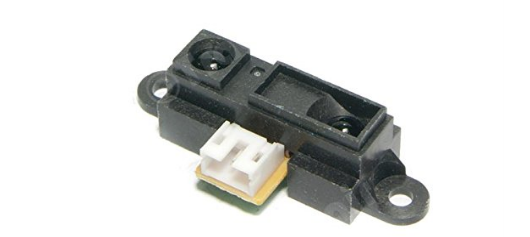
\includegraphics[width=0.6\textwidth]{images/infrarot.png}
	\caption{ \ Infrarot-Sensor  (Quelle: amazon.de)}
	\label{infrarot} % über das label kann man aus dem Text auf das Bild verweisen
\end{figure}
\pagebreak
